\documentclass{article}
\usepackage[utf8]{inputenc}
\usepackage[T1]{fontenc}
\usepackage{graphicx}
\usepackage{hyperref}
\usepackage{geometry}
\geometry{margin=1in}

\title{ERANARCHIA}
\date{Encyclopaedia Britannica (1771)}

\begin{document}
\maketitle

\section*{Historical source}
\textbf{Entry ID:} \texttt{entry-eranarchia-2473} \\
\textbf{Volume ID:} 144133902 \\
\textbf{Character Count:} 493

\subsection*{Extracted Text}
ERANARCHIA, a public officer among the ancient Greek, which bullets was to pedide over and direct the alms and provins made for the poor. Cornelius Nepos, in his lit of Espainindodas, deferibes his office thus; when any period was reduced so poverty, taken captive, or had a daughter to marry, which he could not effect for want of money, etc. the eranarcha call- ed an offender of friends and neighbours, and tax- ed each according to his means and ethars, to contri- bute towards his relief.



\section*{Source record}
\begin{itemize}
\item \textbf{Dataset:} \texttt{NationalLibraryOfScotland/encyclopaedia\_britannica\_illustrated}
\item \textbf{Dataset Revision:} \texttt{309f765b1ecc83e0a7f7762e44b4a927a7555443}
\item \textbf{Page ID:} \texttt{britannica:309f765b1ecc83e0a7f7762e44b4a927a7555443:train:2473} \\
  \textbf{Filename:} \texttt{page-2473-b849fb7f25f2.jpg} \\
  \textbf{Row Index:} 2473 \\
  \textbf{SHA256:} \texttt{b849fb7f25f25b39...}
\end{itemize}

\begin{figure}[h]
\centering
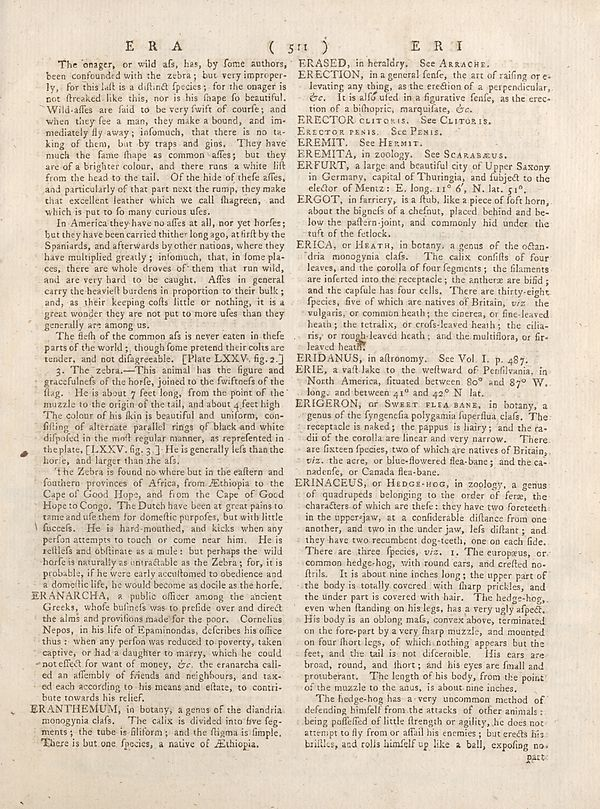
\includegraphics[width=0.85\textwidth]{../scans/page-2473-b849fb7f25f2.jpg}
\caption*{Source scan: \texttt{page-2473-b849fb7f25f2.jpg}}
\end{figure}

\end{document}
